\documentclass{abnt}

\usepackage[utf8]{inputenc}
\usepackage[T1]{fontenc}
\usepackage[brazilian]{babel}
\usepackage[alf]{abntcite}
\usepackage{url}

\ifx\pdftexversion\undefined
\usepackage[dvips]{graphicx}
\else
\usepackage[pdftex]{graphicx}
\usepackage[pdftex,table]{xcolor}
\DeclareGraphicsRule{*}{mps}{*}{}
\fi

\autor{Marcus V. C. Floriano e Debora A. L. Chama}
\titulo{Metadata-based Test Framework to Verify External Effects of the Target Classes}
\orientador{Eduardo M. Guerra}
\instituicao{Aeronautical Institute of Technology \par
Praça Marechal Eduardo Gomes, 50 \par
Vl Acácias - SJ Campos – SP, Brazil}
\local{São Paulo - SP}
\data{03/2012}

\makeindex

\begin{document}

\capa
\folhaderosto

\setlength{\ABNTsignthickness}{1pt}
\begin{folhadeaprovacao}
	Seu texto aqui, onde você deve informar o titulo, data da aprovação (dia, mês e ano), autor do trabalho, local (cidade e estado). E por fim a banca examinadora:
	\assinatura{Prof. fulano \\ Orientador}
	\assinatura{Prof. fulano II \\ Faculdade}
\end{folhadeaprovacao}

\begin{resumo}
	Resumo em português!!!.
\end{resumo}

\begin{abstract}
	Abstract in english!///>>>.
\end{abstract}

\sumario
\listoffigures

%corpo do texto do trabalho 
\chapter{Introdução} 
O trabalho tem como principal objetivo apresentar uma ferramenta baseada em metadados para efeitos externos em testes de unidade. Para isso é apresentando conceitos básicos sobre testes de unidade, bem como a relação e problemas enfrentados com dependências externas e as soluções existentes atualmente.\\
Para entendimento completo é apresentado a solução que foi desenvolvida com base em um padrão para frameworks baseados em meta-dados, a extensão do JUnit4 utilizando a funcionalidade "Runners" e a utilização de Proxy Dinâmico como meio de interceptar as chamadas para os métodos dos testes de unidade.\\

\chapter{Conceitos básicos sobre testes de unidade}



\chapter{Utilizando testes de unidade com dependências externas} 
\chapter{Soluções existentes}
\chapter{Framework baseado em meta-dados}
São frameworks cujo processamento lógico é baseado em meta-dados adicionados nas classes, e as instancias dessas classes trabalham com essa informação. O artigo ``A Pattern Language for Metada-based Frameworks'' \cite{GUERRA-PATTERN} descreve os frameworks que utilizam dessa abordagem, e apresenta um conjunto de padrões cujo o objetivo é a organização do desenvolvimento dessas soluções.\\

Basicamente esse conjunto de padrões é estruturado em Padrões Estruturais, Padrões para Leitura dos Meta-dados e Padrões para o Processamento Lógico.\\

\section{Padrões Estruturais}

Os padrões estruturais estão divididos e dois o ``Metadata Container'' e o ``Metadata Repository'', esses padrões definem como estruturar as classes de um framework baseado em meta-dados, pode-se dizer que esse é a base para do ``Patter Language'' sendo que todos os outros padrões são dependente desses.

O Metadata Container tem o objetivo de separar a leitura dos metas-dados da lógica de execução.


\section{Padrões para Leitura dos Meta-dados}
\section{Padrões para o Processamento Lógico}

\chapter{O framework ``Make a Test''}
\section{JUnit 4 - Runners}
\section{Proxy dinâmicos}
\section{Estrutura do ``Make a Test''}

Para a execução da ferramenta é utilizado a funcionalidade ``Runners'' do JUnit \cite{junit}, assim é possível utilizar todas as funcionalidades do JUnit e adicionar as novas dessa ferramenta.

O Proxy dinâmico facilita a forma de interceptar as chamadas para os métodos das classes de testes de unidade, a fim de permitir a injeção de comportamentos para verificar os efeitos externos.

A estrutura do ``Make a Test'' está baseada em um ``Pattern Language'' para frameworks baseados em meta-dados \cite{GUERRA-PATTERN}, conforme descrito anteriormente em maiores detalhes.

A utilização da ferramenta nas classes de testes de unidade são feitas a partir de anotações e das classes executoras dessas anotações.

\subsection{Runners}

Runners é a forma de adicionar funcionalidade ao JUnit.

\begin{figure}[!ht]
	\centering
	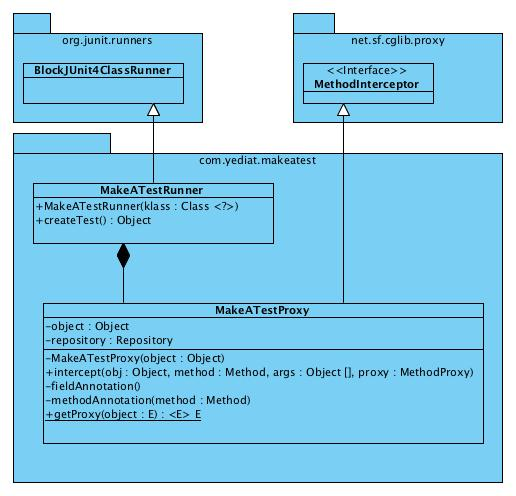
\includegraphics[scale=0.50]{uml/runners.jpg}
	\caption{Estrutura de classes que representa a extensão do BlockJUnit4ClassRunner, e a implementação MethodInterface para a criação do Proxy.}
	\label{uml-class-runners}
\end{figure}

\subsection{Proxy dinâmico}

\subsection{Pattern Language}

\begin{figure}[!ht]
	\centering
	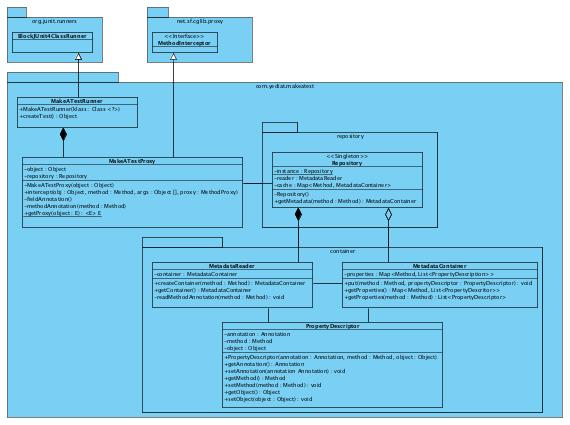
\includegraphics[scale=0.70]{uml/makeatest.jpg}
	\caption{Estrutura de classes do ``Make a Test''.}
	\label{uml-class-makeatest}
\end{figure}


\subsubsection{Padrões Estruturais}



\subsubsection{Padrões para Leitura dos Meta-Dados}
\subsubsection{Padrões para Processamento Lógico}

\subsection{Anotações e Configurações}





\subsection{Metada Container}
MakeATestRunner
MakeATestProxy
MetadataReader
MetadataContainer


Primeiro é criado um Descriptor que representa as anotações em valores, Propertie Description e Comparison Descriptor.\\
Um PropertieDescription representa um unico valore, o ComparisonDescriptor representa um conjunto de PropertieDescription.\\

O ComparisonMetadataReader cria o conjunto de valores para o ComparisonDescriptor a partir de uma objeto do tipo CLASS.\\

O ComparisonComponent recupera o ComparisonMetadataReader para recuperar os valores.\\

O Repositorio é utilizado para criar uma unica instancia, que é utilizado o padrão singleton, no Repositorio são criados o ComparisonMetadataReader e um cache que é formado por um hashmap e a chave é a CLASS que contêm as anotações.


\bibliography{makeatest}

\end{document}